\documentclass[14pt]{extarticle}
\usepackage[margin = 1in]{geometry}
\usepackage{graphicx}
\begin{document}
\begin{Large}
\begin{center}
\textbf{PROJECT SYNOPSIS}
\end{center}
\end{Large}

\section{Synopsis}
\subsection{Introduction}
{\quad}Machine vision (MV) is the technology and methods used to provide imaging-based automatic inspection and analysis for such applications as automatic inspection, process control, and robot guidance, usually in industry. The main task of machine vision systems is providing computer understandable descriptions of objects from either single image or whole array of images. One such area of application  is in automated visual product inspection. An automated visual inspection system must discover and classify possible defects from product images and should be fairly quick and robust. These requirements are needed if automated systems are to replace human inspection which has many drawbacks, mainly caused by tiredness and slowness (modern production methods usually facilitate productions speeds humans can't cope with). Such an automated system can be assembled with the digital image processing at its core in order to detect dimensional  defects in large scale manufacturing industries.\\

{\quad}Digital Image Processing focuses on developing a computer system that is able to perform processing on an image. The input of that system is a digital image and the system process that image using efficient algorithms, and gives an image as an output. In DIP,  Pixel subtraction is one of the methods where the digital numeric value of one pixel or whole image is subtracted from another image. This is primarily done for one of two reasons – leveling uneven sections of an image such as half an image having a shadow on it, or detecting changes between two images.[1] This detection of changes can be used to tell if something  in the image varies and this is the basis for defect detection.



\subsection{Motivation:}
{\quad}In most of the manufacturing industries, it is common to obtain a few defective products among the perfect ones. On a large scale, it is quite complex to accurately detect a defective product.\\

{\quad}Defects in manufacturing occur when a product is improperly manufactured and departs from its intended design. One of the common defects in a product is dimensional inaccuracy. Conventionally, there are two ways to detect such inaccuracies. The first one is to do a quality control check performed by humans. But this is tedious, slow and also prone to errors. The second method is to use devices which can automatically detect such anomalies. But such devices are expensive and are mostly employed in later stages of manufacturing.\\

{\quad}Hence there is a need for detecting these defects in a cost-effective and efficient manner in early stages of manufacturing.


\subsection{Problem Statement:}
{\quad}An automated system is to be assembled which can detect and label the dimensional defects of a given object. Such a system must  perform with a high degree of accuracy and also be cost-effective. The designed system must also be easy to operate so that it is deploy-able in a production line with relative ease.

\subsection{Objective:}
{\quad}This work presents a new, real-time, highly automated tool for defect detection based on the combination of statistical and Image Processing approach.The specific goals of this investigation are to develop an efficient non-intrusive, online dimensional defect detection. These are achieved by creating a machine-vision system able to perform real time acquisition,  image processing and classification. The automatic inspection system will allow the detection and classification of the most frequently occurring dimensional defects in the manufactured products while storing and displaying the possible solutions to the user.

\subsection{Block Diagram:}

\begin{figure}[h]
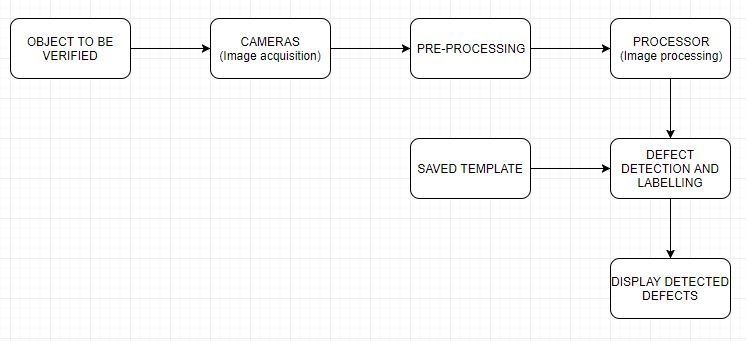
\includegraphics[scale=1]{bd.jpg}
\caption{Basic Block Diagram}
\end{figure}

{\quad}A basic block diagram of the proposed project is given above. The first step is to acquire the image of the object. Since the object can have defects along any axis, we will take multiple images of the object from different angles. These bunch of images are sent to a processor, which will use image processing techniques to enhance and find the defects in the object by comparing it with a previously saved template of the object. The defects, if found, are then stored and displayed to the user in the last step. 

\subsection{Project Outcome:}
{\quad}The designed automated system will be able to take pictures of the object in all the 3 dimensions using cameras and process the images using image processing techniques. The system will compare the processed image with an initially stored reference image of the same and detect abnormalities or flaws, if any. Finally it will display the area or the part where defect is present and suggest an alternative method for resolving the flaw or problem. 

\subsection{Application:}
\begin{itemize}
\item{
Although the system is limited to only manufacturing industries, it plays a vital role in quality control of the goods manufactured.
}
\item{
If such a system is employed in early stages of production, it can be used to detect the faulty goods beforehand and have a better chance of rectifying the errors, thus reducing wastage.
}
\item{
It can be used in 3D printing and CNC machining to check if there is any defects in the printed materials.
}
\item{
It can be used to check the dimensions of an unknown object.
}

\end{itemize}

\section{Literature Survey:}
\subsection{Software Requirements:}
\subsubsection{OpenCV:}
{\quad}OpenCV (Open Source Computer Vision) is a library of programming functions mainly aimed at real-time computer vision. It was originally developed by Intel and is released under BSD license. Hence it is free for both academic and commercial purposes.  It has C++, C, Python and Java interfaces and supports Windows, Linux, Mac OS, iOS and Android. OpenCV was designed for computational efficiency and with a strong focus on real-time applications. Written in optimized C/C++, the library can take advantage of multi-core processing. Enabled with OpenCL, it can take advantage of the hardware acceleration of the underlying heterogeneous compute platform.

\subsubsection{Arduino IDE:}
{\quad}The Arduino project provides the Arduino integrated development environment (IDE), which is a cross-platform application written in the programming language Java. It originated from the IDE for the languages Processing and Wiring. It includes a code editor with features such as text cutting and pasting, searching and replacing text, automatic indenting, brace matching, and syntax highlighting, and provides simple one-click mechanisms to compile and upload programs to an Arduino board. It also contains a message area, a text console, a toolbar with buttons for common functions and a hierarchy of operation menus.\\

{\quad}The Arduino IDE supports the languages C and C++ using special rules of code structuring. The Arduino IDE supplies a software library from the Wiring project, which provides many common input and output procedures. User-written code only requires two basic functions, for starting the sketch and the main program loop, that are compiled and linked with a program stub main() into an executable cyclic executive program with the GNU tool-chain, also included with the IDE distribution. The Arduino IDE employs the program avrdude to convert the executable code into a text file in hexadecimal encoding that is loaded into the Arduino board by a loader program in the board's firmware.

\subsubsection{Python:}
{\quad}Python is a widely used high-level programming language for general-purpose programming.Python has a design philosophy that emphasizes code readability and a syntax that allows programmers to express concepts in fewer lines of code than might be used in languages such as C++ or Java.The language provides constructs intended to enable writing clear programs on both a small and large scale.Python features a dynamic type system and automatic memory management and supports multiple programming paradigms, including object-oriented, imperative, functional programming, and procedural styles. Python can be run on variety of OS like Windows, macOS, Linux and even Raspbian.


\subsection{Hardware Requirements:}
\subsubsection{Arduino Uno:}
{\quad}The Arduino Uno is a micro-controller board based on the ATmega328 (data-sheet). It has 14 digital input/output pins (of which 6 can be used as PWM outputs), 6 analog inputs, a 16 MHz crystal oscillator, a USB connection, a power jack, an ICSP header, and a reset button. It contains everything needed to support the micro-controller; simply connect it to a computer with a USB cable or power it with a AC-to-DC adapter or battery to get started.
The Uno differs from all preceding boards in that it does not use the FTDI USB-to-serial driver chip. Instead, it features the Atmega16U2 (Atmega8U2 up to version R2) programmed as a USB-to-serial converter.

\subsubsection{Raspberry Pi:}
{\quad}Raspberry Pi is an ARM based credit card sized SBC(Single Board Computer) created by Raspberry Pi Foundation. Raspberry Pi runs Debian based GNU/Linux operating system Raspbian and ports of many other OSes exist for this SBC.
The Raspberry Pi 3 Model B is the third generation Raspberry Pi. This powerful credit-card sized single board computer can be used for many applications and supersedes the original Raspberry Pi Model B+ and Raspberry Pi 2 Model B.
Additionally it adds wireless LAN and Bluetooth connectivity making it the ideal solution for powerful connected designs.

\subsubsection{Camera module:}
{\quad}The Raspberry Pi camera module can be used to take high-definition video, as well as stills photographs. The camera consists of a small (25mm by 20mm by 9mm) circuit board, which connects to the Raspberry Pi's Camera Serial Interface (CSI) bus connector via a flexible ribbon cable. The camera's image sensor has a native resolution of five megapixels and has a fixed focus lens. The software for the camera supports full resolution still images up to 2592x1944 and video resolutions of 1080p30, 720p60 and 640x480p60/90.

\end{document}
